\documentclass[10pt,pdf,hyperref={unicode}]{beamer}% тип документа
% далее идёт преамбула
\usepackage{tikz}
\usetikzlibrary{graphs}
\usepackage[T1,T2A]{fontenc}
\usepackage[utf8]{inputenc}
\usepackage[english,russian]{babel}
%\usepackage{amsmath}
%\usepackage{amsfonts}
%\usepackage{amssymb}
%\usepackage{makeidx}

\usepackage[english,russian]{babel}
\usetheme{Berlin}

\title{Технология программирования}
\author{Романцов Григорий Дмитриевич}
\date{}

\begin{document}% начало презентации

\begin{frame}% первый слайд
  \titlepage
\end{frame}

\begin{frame}{Отладка ПО}
Отладка — это  процесс  определения  и  устранения  причин ошибок.  Этим  она  отличается  от  тестирования,  направленного на обнаружение ошибок. В
некоторых проектах отладказанимает  до  50\%  общего  времени  разработки. Многие  программисты считают отладку самым трудным аспектом программирования.
\end{frame}

\begin{frame}{Отладка ПО}

  \begin{figure}[h]

    \center{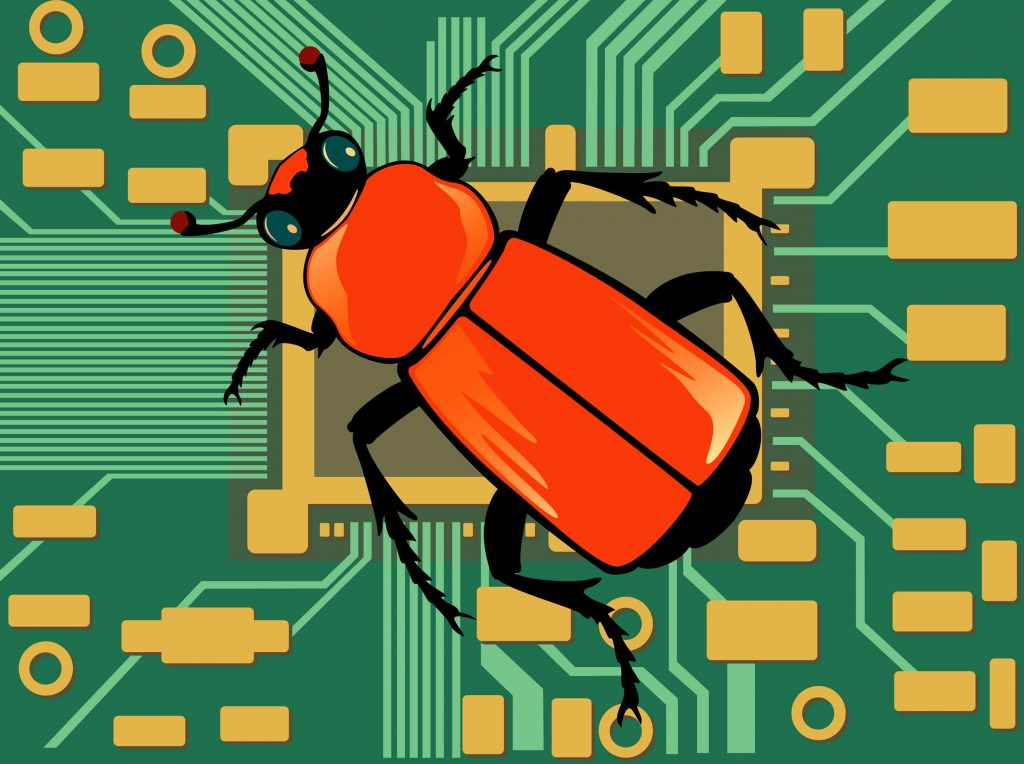
\includegraphics[width=\textwidth]{bug.jpg}}

  \end{figure}

\end{frame}

\begin{frame}{Дефекты как возможности обучения}

  \begin{itemize}

    \item {\bfИзучить  программу,  над  которой  работаете}
    \item {\bfИзучить собственные ошибки}
    \item {\bfИзучить качество своего кода с точки зрения}
    \item {\bfИзучить  используемые  способы  решения  проблем}
    \item {\bfИзучить используемые способы исправления дефектов}

  \end{itemize}
\end{frame}

\begin{frame}{Неэффективный подход}
        \begin{itemize}
          \item {\bfПоиск  дефектов,  основанный  на  гадании}
          \item {\bfТщательный анализ проблемы — пустая трата времени}
        \end{itemize}
\end{frame}

\begin{frame}{Научный метод}

  \begin{enumerate}
  \item Сбор  данных  при  помощи  повторяющихся  экспериментов.
  \item Формулирование  гипотезы,  объясняющей  релевантные  данные.
  \item Разработка  эксперимента,  призванного  подтвердить  или  опровергнуть  гипотезу.
  \item Подтверждение  или  опровержение  гипотезы.
  \item Повторение  процесса  в  случае  надобности
\end{enumerate}


\end{frame}

\begin{frame}{Научный метод отладки}

  \begin{enumerate}
  \item Стабилизация  ошибки.
  \item Определение  источника  ошибки.
        \begin{enumerate}
          \item Сбор  данных,  приводящих  к  дефекту.
          \item Анализ собранных данных и формулирование гипотезы, объясняющей дефект.
          \item Определение  способа  подтверждения  или  опровержения  гипотезы,  основанного  или  на  тестировании  программы,  или  на  изучении  кода.
          \item Подтверждение  или  опровержение  гипотезы  при  помощи  процедуры,определенной  в  п. 2(c).
        \end{enumerate}
  \item Исправление  дефекта.
  \item Тестирование  исправления.
  \item Поиск  похожих  ошибок.
\end{enumerate}

\end{frame}

\begin{frame}{Стабилизация ошибки}
\begin{tabular}{lr}
Александ Александрович & 20,324 \\
Гарри Поттер               &   10,666 \\
Михаил Милый           &  100,788 \\
Мария-Тереза Михельсон           &   88,889 \\
Сендвич Сладкий      &   40,000 \\
Ярило Яркий           &   70,860 \\
\end{tabular}
\end{frame}


\begin{frame}{Стабилизация ошибки II}
\begin{tabular}{lr}
Александ Александрович & 20,324 \\
Гарри Поттер               &   10,666 \\
Мария-Тереза Михельсон           &   88,889 \\
Михаил Милый           &  100,788 \\
Сендвич Сладкий      &   40,000 \\
Ярило Яркий           &   70,860 \\
\end{tabular}
\end{frame}

\begin{frame}{Стабилизация ошибки III}

\begin{tabular}{lr}
Александ Александрович & 20,324 \\
Ар-Истарх Аристархович  &   50,877 \\
Гарри Поттер               &   10,666 \\
Максим Малый           &   88,889 \\
Михаил Милый           &  100,788 \\
Сендвич Сладкий      &   40,000 \\
Ярило Яркий           &   70,860 \\
\end{tabular}

\end{frame}


\begin{frame}{Определение источника ошибки}
\begin{tabular}{lr}
Александ Александрович & 20,324 \\
Ар-Истарх Аристархович  &   50,877 \\
Гарри Поттер               &   10,666 \\
Иван Иванов           & 40,323\\
Мария-Тереза Михельсон           &   88,889 \\
Михаил Милый           &  100,788 \\
Сендвич Сладкий      &   40,000 \\
Ярило Яркий           &   70,860 \\
\end{tabular}
\end{frame}


\begin{frame}{Советы по поиску причин дефектов}

  \begin{itemize}

    \item {\bfФормулируя  гипотезу,  используйте  все  имеющиеся  данные}
    \item {\bfДетализируйте тесты, приводящие к ошибке}
    \item {\bfПроверяйте код при помощи блочных тестов}
    \item {\bfИспользуйте  разные  инструменты}
    \item {\bfВоспроизведите  ошибку  несколькими  способами}
    \item {\bfГенерируйте больше данных для формулирования большего числа гипотез}
    \item {\bfИспользуйте  результаты  отрицательных  тестов}
    \item {\bfИспользуйте  «мозговой  штурм»  для  построения  нескольких  гипотез}
    \item {\bfСоставьте  список  подходов,  которые  стоит  попробовать}
    \item {\bfСократите  подозрительную  область  кода}
    \item {\bfС  подозрением  относитесь  к  классам  и  методам,  которые содержали дефекты ранее}
    \item {\bfПроверьте  код,  который  был  изменен  недавно}
    \item {\bfРасширьте подозрительный фрагмент кода}
    \item {\bfВыполняйте интеграцию инкрементно}
  \end{itemize}

\end{frame}

\begin{frame}{Стандартыне техники отладки}

  \begin{enumerate}
  \item Отладка с помощью дебаггера.
  \item Отладка с помощью зрительного анализа кода.
  \item Отладка с помощью прототипирования.
  \item Профилирование кода.
  \item Выполнение кода в другой среде.
  \item Отладка с помощью RPC.
  \item Отладка путем анализа документации и файлов проекта.
  \item Отладка трансляцией кода.
  \item Отладка разработкой интерпретатора.
\end{enumerate}

\end{frame}


\begin{frame}{Архитектура ПО}
  \begin{figure}[h]
    \center{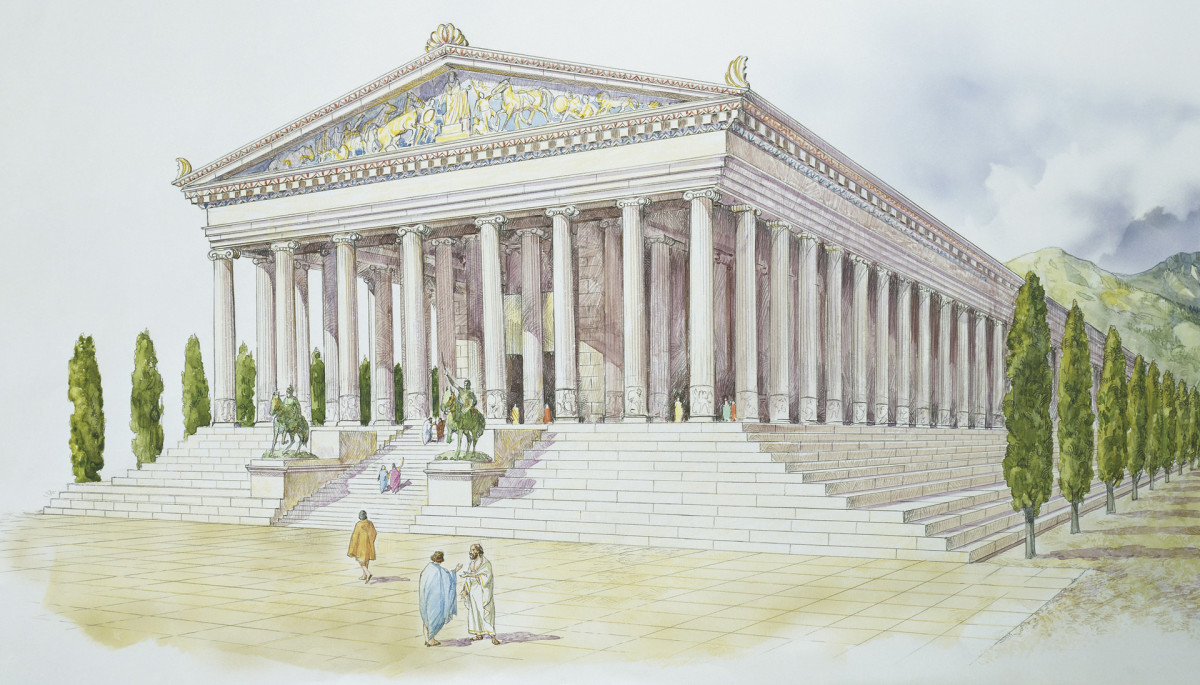
\includegraphics[width=\textwidth]{arh.jpg}}
  \end{figure}
\end{frame}

\begin{frame}{Критерии хорошей архитектуры}
  \begin{itemize}
    \item \textbf{Эффективность системы.}
    \item \textbf{Гибкость системы.}
    \item \textbf{Расширяемость системы.}
    \item \textbf{Масштабируемость процесса разработки.}
    \item \textbf{Тестируемость.}
    \item \textbf{Возможность повторного использования.}
    \item \textbf{Хорошо структурированный, читаемый и понятный код.}
  \end{itemize}
\end{frame}

\begin{frame}{Модульная архитектура. Декомпозиция как основа}
\begin{itemize}
    \item \textbf{Масштабируемость (Scalability)}
    возможность расширять систему и увеличивать ее производительность, за счет добавления новых модулей.
    \item \textbf{Ремонтопригодность (Maintainability)}
    изменение одного модуля не требует изменения других модулей
    \item \textbf{Заменимость модулей (Swappability)}
    модуль легко заменить на другой
    \item \textbf{Возможность тестирования (Unit Testing)}
    модуль можно отсоединить от всех остальных и протестировать / починить
    \item \textbf{Переиспользование (Reusability)}
    модуль может быть переиспользован в других программах и другом окружении
    \item \textbf{Сопровождаемость (Maintenance)}
    разбитую на модули программу легче понимать и сопровождать
\end{itemize}

\end{frame}

\begin{frame}{}
  \begin{figure}[h]
    \center{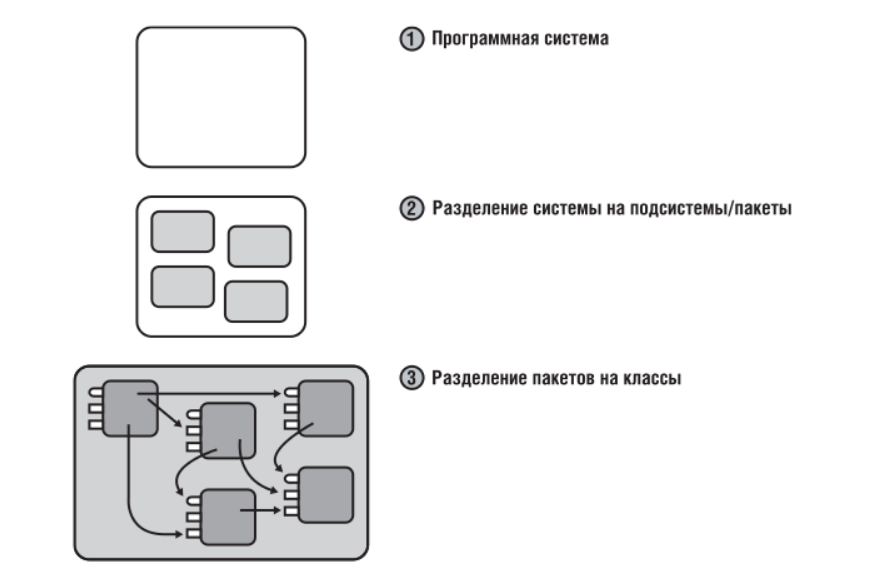
\includegraphics[width=\textwidth]{a2.png}}
  \end{figure}
\end{frame}

\begin{frame}{Как ослаблять связанность между модулями}

\begin{figure}[h]
\center{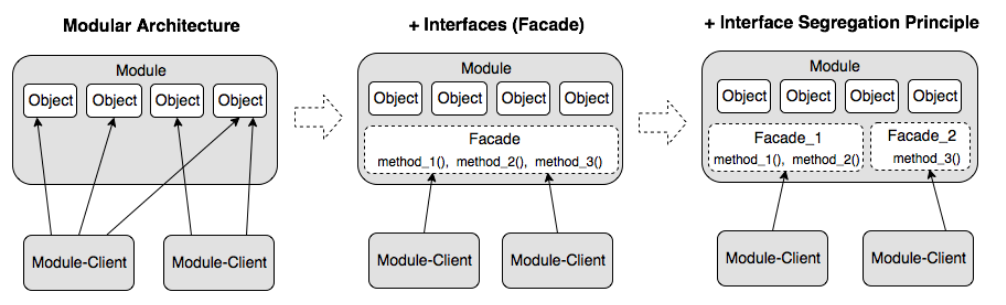
\includegraphics[width=\textwidth]{a3.png}}
\end{figure}

\end{frame}

\begin{frame}{SOLID}
\begin{itemize}
    \item S:\@Single Responsibility Principle (Принцип единственной ответственности).
    \item O:\@ Open-Closed Principle (Принцип открытости-закрытости).
    \item L:\@Liskov Substitution Principle (Принцип подстановки Барбары Лисков).
    \item I:\@Interface Segregation Principle (Принцип разделения интерфейса).
    \item D:\@Dependency Inversion Principle (Принцип инверсии зависимостей).
\end{itemize}
\end{frame}

\begin{frame}{Принцип единой ответственности}
\begin{figure}[h]
\center{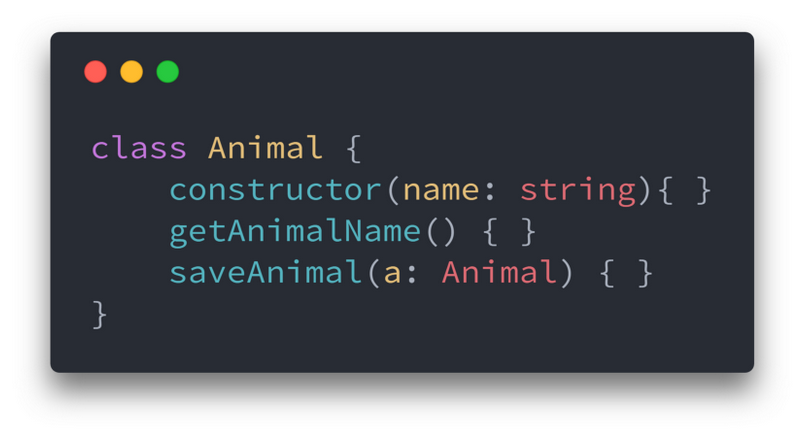
\includegraphics[width=\textwidth]{l1.png}}
\end{figure}
\end{frame}

\begin{frame}{Принцип единой ответственности II}
\begin{figure}[h]
\center{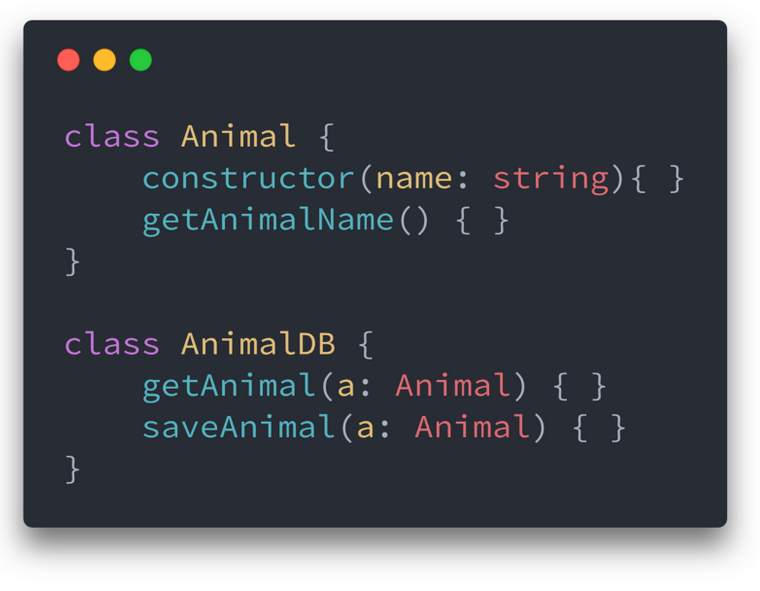
\includegraphics[width=\textwidth]{l2.png}}
\end{figure}
\end{frame}


\begin{frame}{Принцип открытости-закрытости}
\begin{figure}[h]
\center{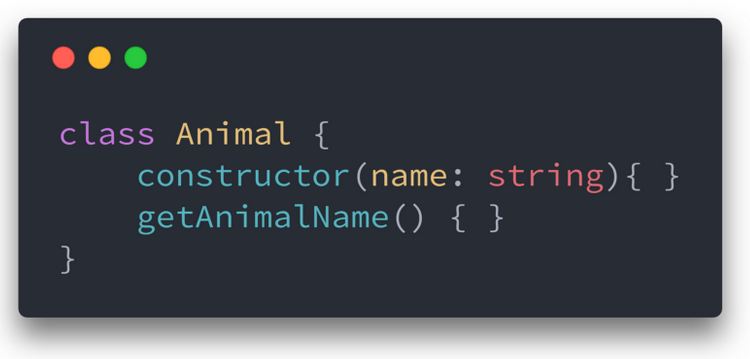
\includegraphics[width=\textwidth]{l3.png}}
\end{figure}
\end{frame}


\begin{frame}{Принцип открытости-закрытости}
\begin{figure}[h]
\center{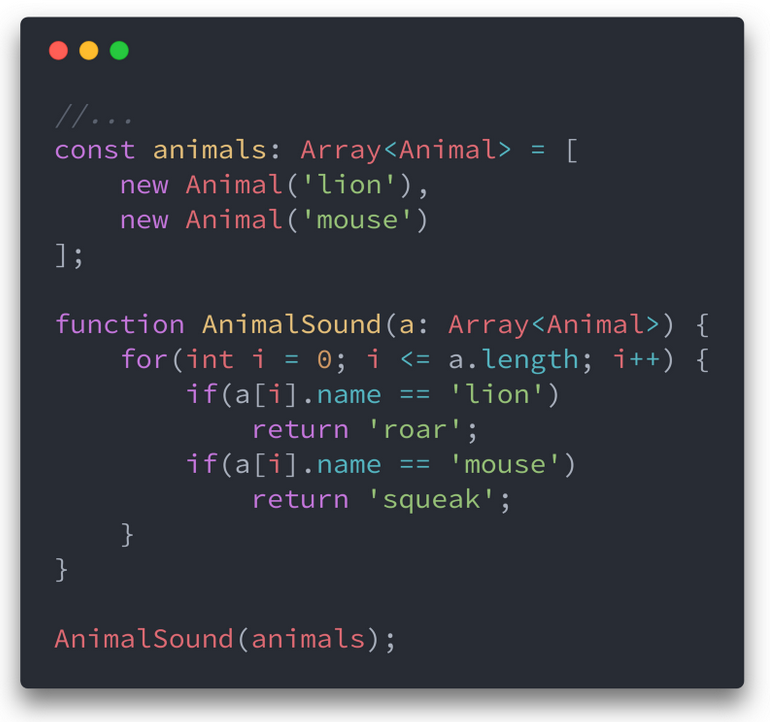
\includegraphics[width=\textwidth]{l4.png}}
\end{figure}
\end{frame}


\begin{frame}{Принцип открытости-закрытости}
\begin{figure}[h]
\center{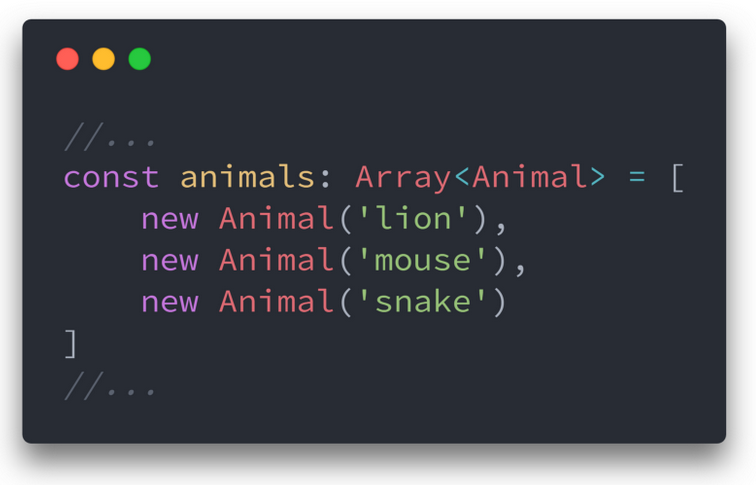
\includegraphics[width=\textwidth]{l5.png}}
\end{figure}
\end{frame}


\begin{frame}{Принцип открытости-закрытости}
\begin{figure}[h]
\center{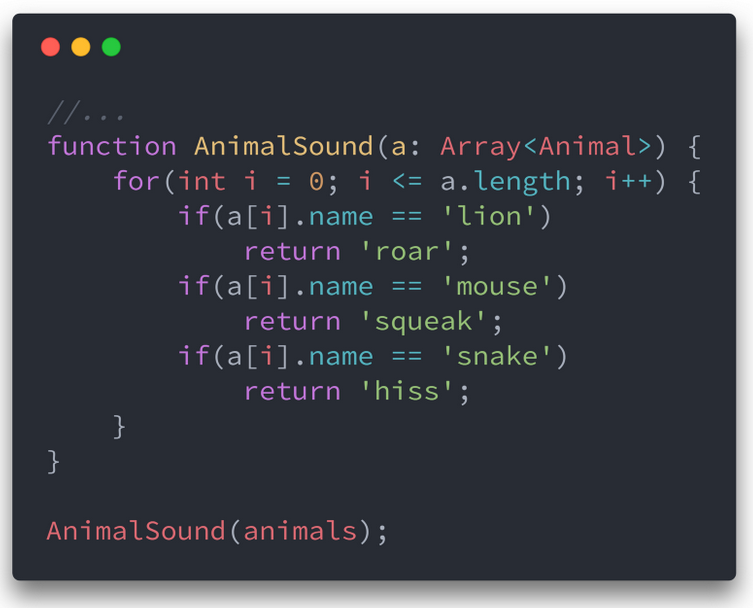
\includegraphics[width=\textwidth]{l6.png}}
\end{figure}
\end{frame}


\begin{frame}{Принцип открытости-закрытости}
\begin{figure}[h]
\center{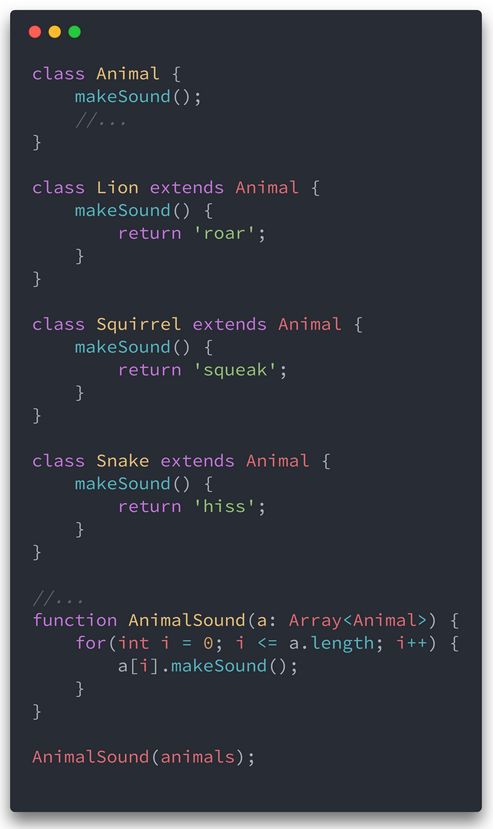
\includegraphics[width=\textwidth]{l7.png}}
\end{figure}
\end{frame}


\begin{frame}{Принцип открытости-закрытости}
\begin{figure}[h]
\center{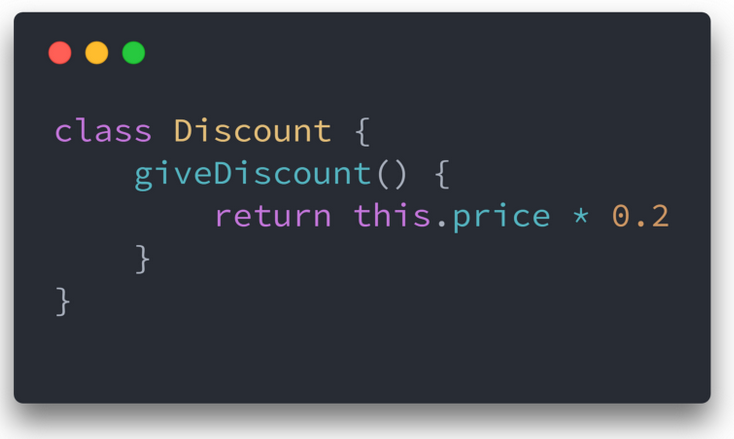
\includegraphics[width=\textwidth]{l8.png}}
\end{figure}
\end{frame}


\begin{frame}{Принцип открытости-закрытости}
\begin{figure}[h]
\center{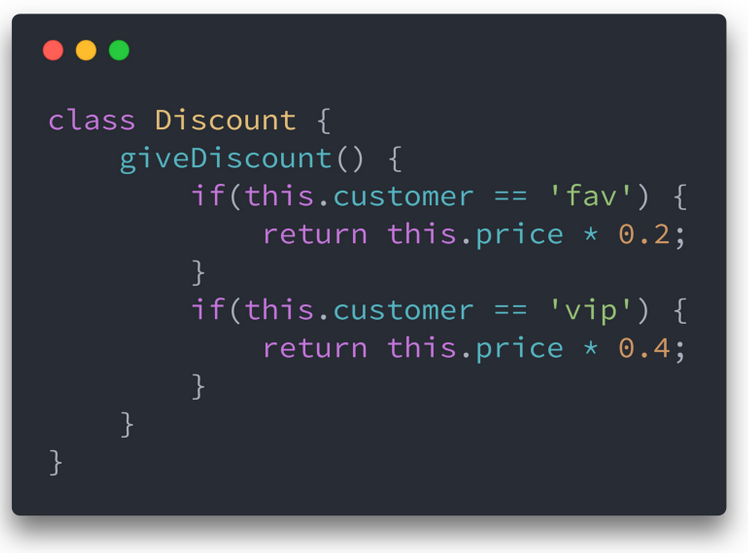
\includegraphics[width=\textwidth]{l9.png}}
\end{figure}
\end{frame}


\begin{frame}{Принцип открытости-закрытости}
\begin{figure}[h]
\center{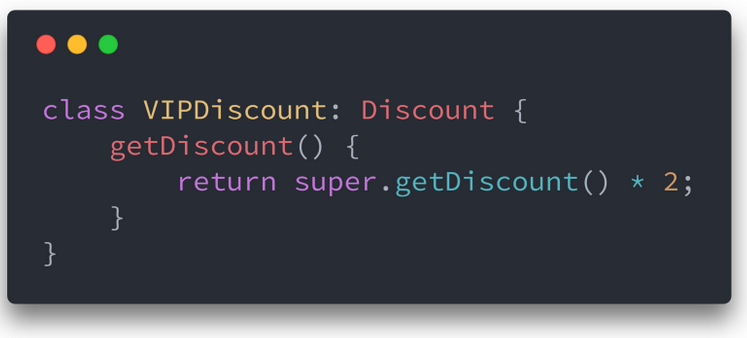
\includegraphics[width=\textwidth]{l10.png}}
\end{figure}
\end{frame}


\begin{frame}{Принцип открытости-закрытости}
\begin{figure}[h]
\center{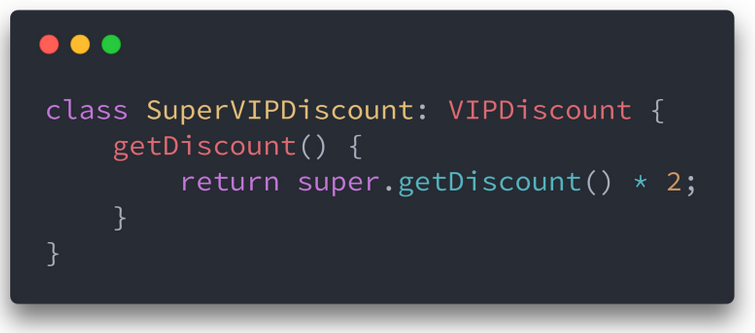
\includegraphics[width=\textwidth]{l11.png}}
\end{figure}
\end{frame}

\begin{frame}{Принцип подстановки Барбары Лиско}
\begin{figure}[h]
\center{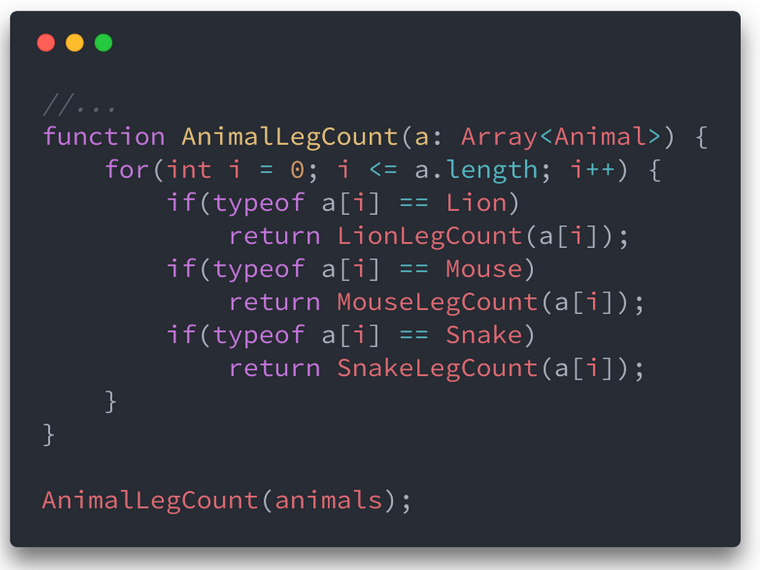
\includegraphics[width=\textwidth]{l12.png}}
\end{figure}
\end{frame}


\begin{frame}{Принцип подстановки Барбары Лиско}
\begin{figure}[h]
\center{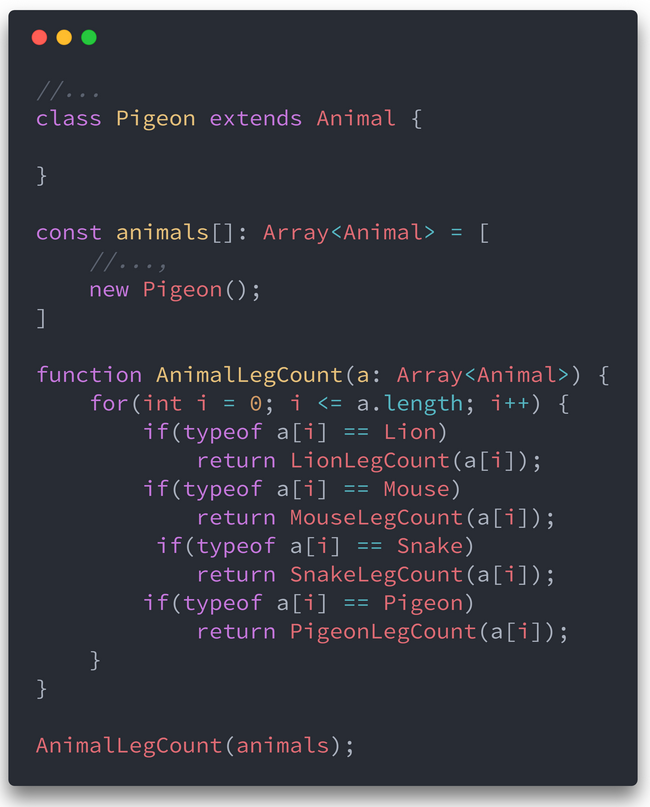
\includegraphics[width=\textwidth]{l13.png}}
\end{figure}
\end{frame}


\begin{frame}{Принцип подстановки Барбары Лиско}
\begin{figure}[h]
\center{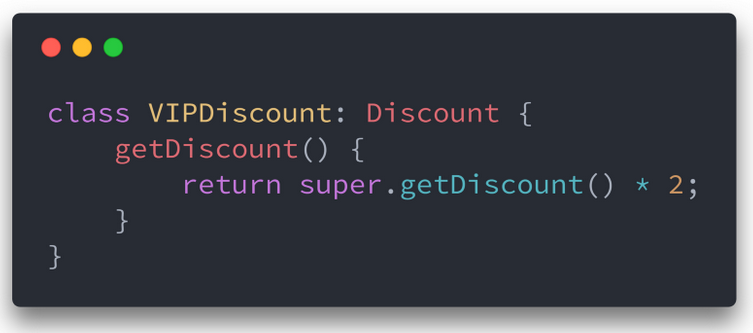
\includegraphics[width=\textwidth]{l14.png}}
\end{figure}
\end{frame}


\begin{frame}{Принцип подстановки Барбары Лиско}
\begin{figure}[h]
\center{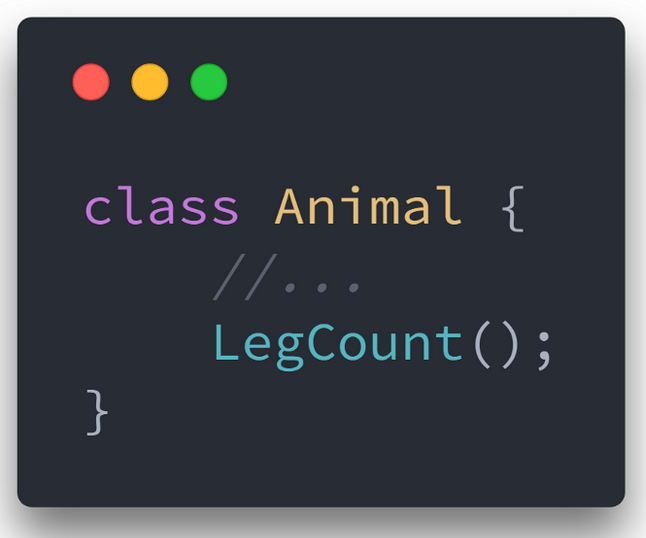
\includegraphics[width=\textwidth]{l15.png}}
\end{figure}
\end{frame}


\begin{frame}{Принцип подстановки Барбары Лиско}
\begin{figure}[h]
\center{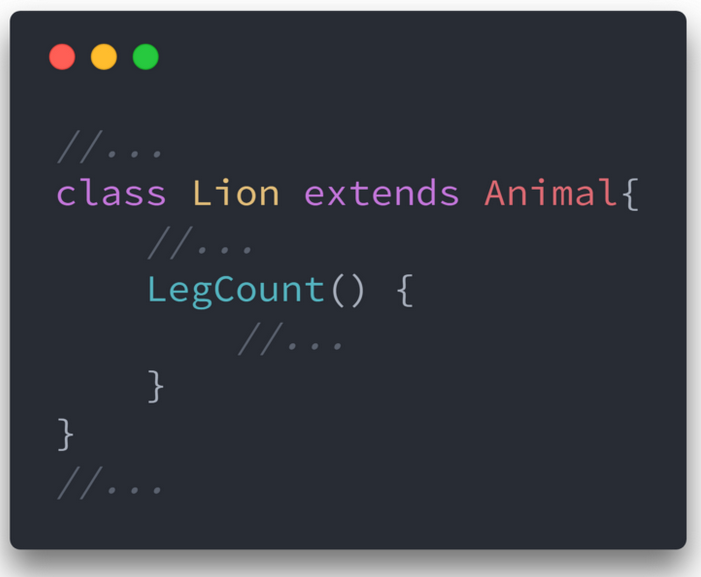
\includegraphics[width=\textwidth]{l16.png}}
\end{figure}
\end{frame}

\begin{frame}{Принцип разделения интерфейса}
\begin{figure}[h]
\center{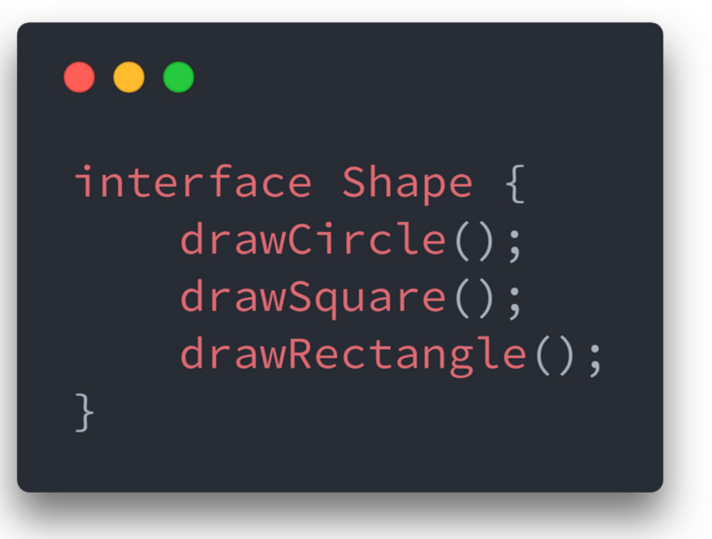
\includegraphics[width=\textwidth]{l17.png}}
\end{figure}
\end{frame}


\begin{frame}{Принцип разделения интерфейса}
\begin{figure}[h]
\center{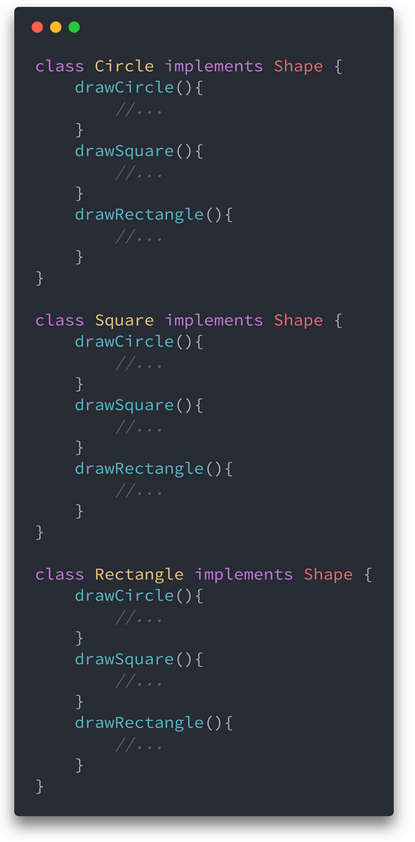
\includegraphics[width=\textwidth]{l18.png}}
\end{figure}
\end{frame}


\begin{frame}{Принцип разделения интерфейса}
\begin{figure}[h]
\center{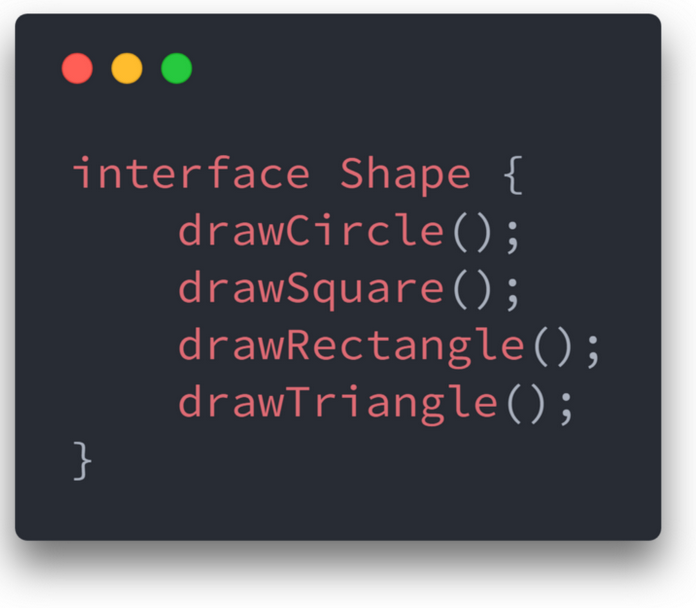
\includegraphics[width=\textwidth]{l19.png}}
\end{figure}
\end{frame}


\begin{frame}{Принцип разделения интерфейса}
\begin{figure}[h]
\center{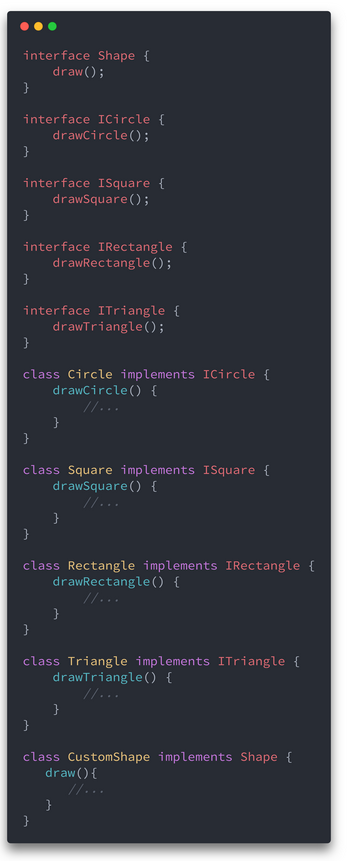
\includegraphics[width=\textwidth]{l20.png}}
\end{figure}
\end{frame}


\begin{frame}{Принцип инверсии зависимостей}
\begin{figure}[h]
\center{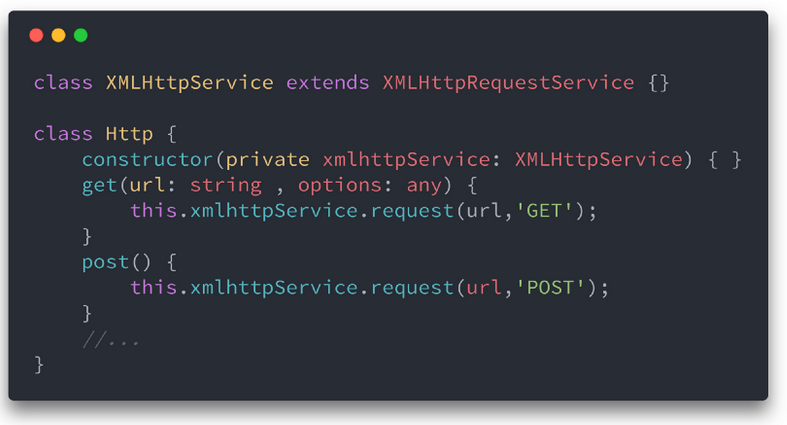
\includegraphics[width=\textwidth]{l21.png}}
\end{figure}
\end{frame}


\begin{frame}{Принцип инверсии зависимостей}
\begin{figure}[h]
\center{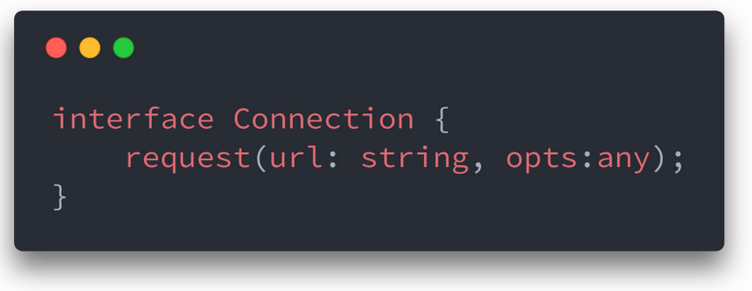
\includegraphics[width=\textwidth]{l22.png}}
\end{figure}
\end{frame}


\begin{frame}{Принцип инверсии зависимостей}
\begin{figure}[h]
\center{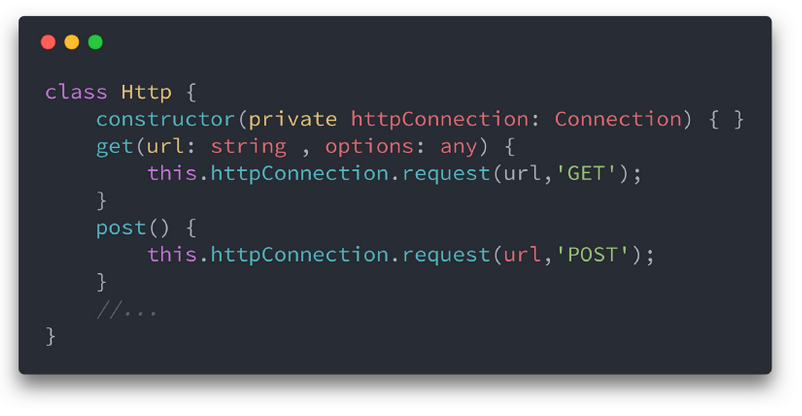
\includegraphics[width=\textwidth]{l23.png}}
\end{figure}
\end{frame}


\begin{frame}{Принцип инверсии зависимостей}
\begin{figure}[h]
\center{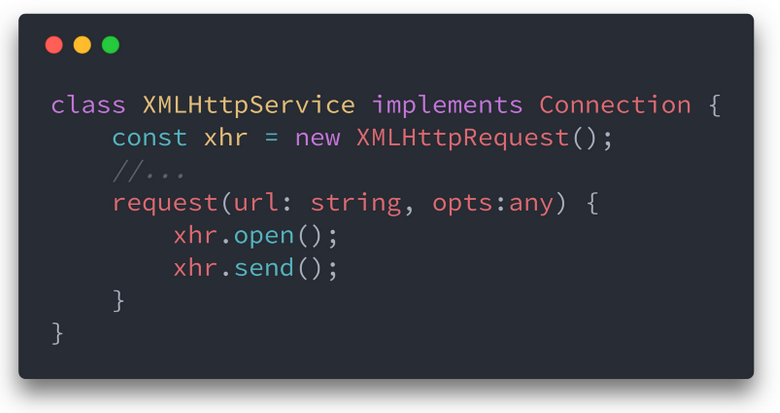
\includegraphics[width=\textwidth]{l24.png}}
\end{figure}
\end{frame}


\begin{frame}{Принцип инверсии зависимостей}
\begin{figure}[h]
\center{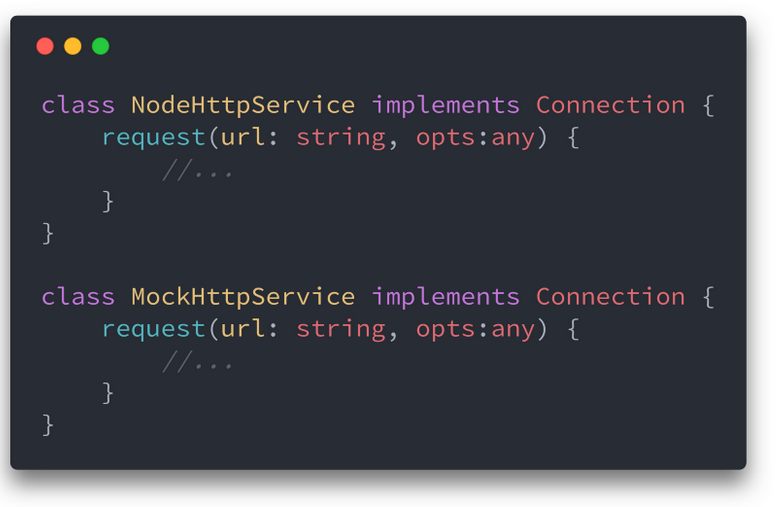
\includegraphics[width=\textwidth]{l25.png}}
\end{figure}
\end{frame}

\begin{frame}{}
\begin{figure}[h]
\center{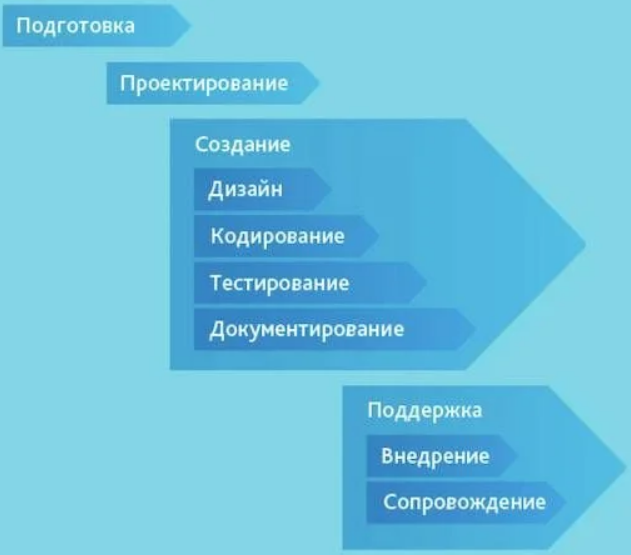
\includegraphics[width=\textwidth]{m1.png}}
\end{figure}
\end{frame}

\begin{frame}{}
\begin{figure}[h]
\center{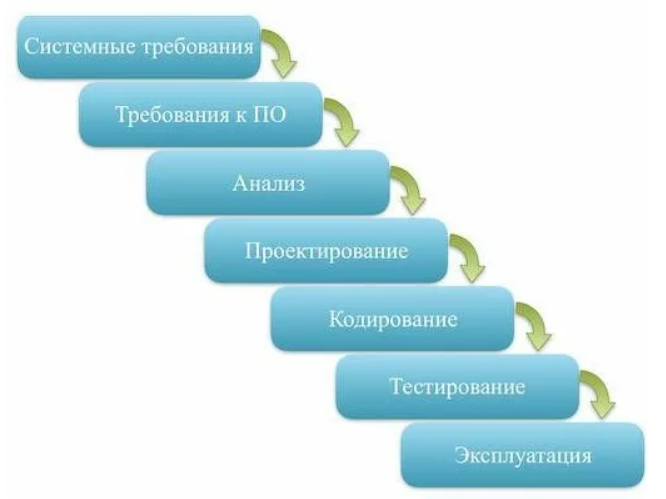
\includegraphics[width=\textwidth]{m2.png}}
\end{figure}
\end{frame}

\begin{frame}{}
\begin{figure}[h]
\center{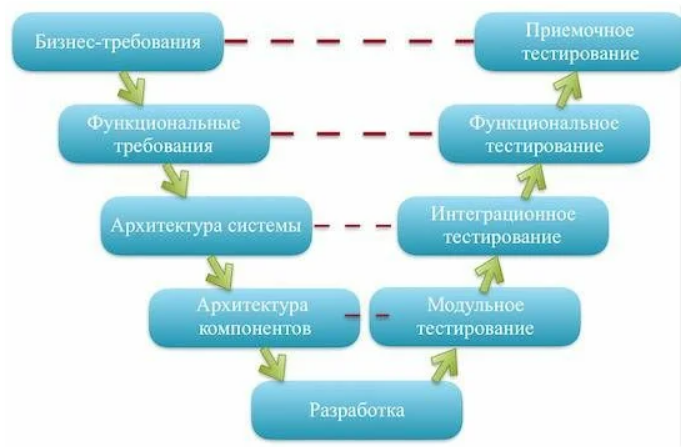
\includegraphics[width=\textwidth]{m3.png}}
\end{figure}
\end{frame}

\begin{frame}{}
\begin{figure}[h]
\center{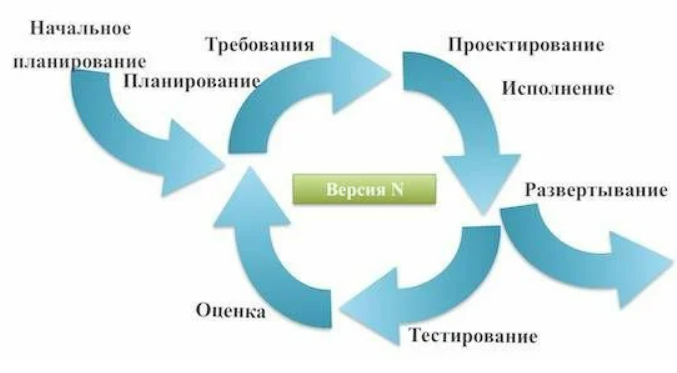
\includegraphics[width=\textwidth]{m4.png}}
\end{figure}
\end{frame}

\begin{frame}{}
\begin{figure}[h]
\center{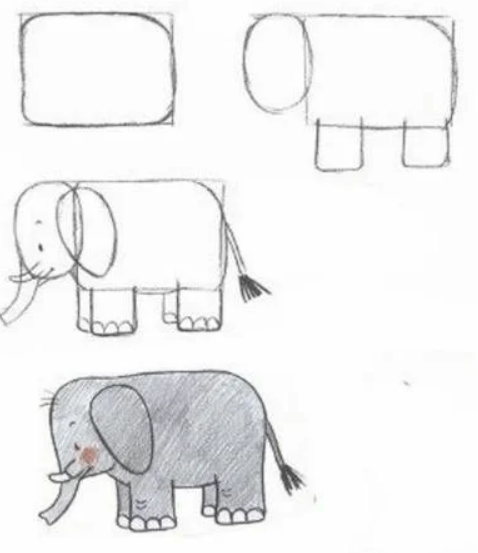
\includegraphics[width=\textwidth]{m5.png}}
\end{figure}
\end{frame}

\begin{frame}{}
\begin{figure}[h]
\center{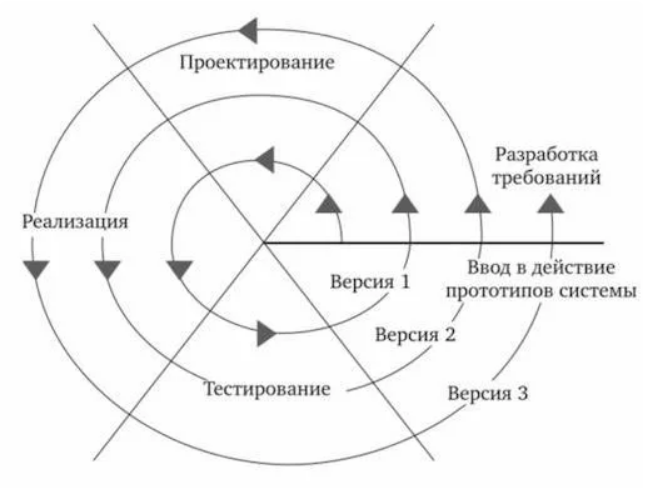
\includegraphics[width=\textwidth]{m6.png}}
\end{figure}
\end{frame}

\end{document}
